%%%%%%%%%%%%%%%%%%%%%%%%%%%%%%%%%%%%%%%
%----------------------------------------     统计检验     ---------------------------------------%
%%%%%%%%%%%%%%%%%%%%%%%%%%%%%%%%%%%%%%%
\chapter{统计检验}
本章将主要关注本文的研究背景——第三方库与移动应用的关系,从统计学角度,对现实中的数据进行统计分析和检验验证。本文从Google Play上爬取了28,261个移动应用以及他们的评分信息。为了深入研究是否使用第三方库与移动应用成功与否的关系,本文将围绕以下研究问题来展开:\textbf{使用第三方库的移动应用是否有更高的评分?}因为使用第三方库可以减少开发者实现相应功能的时间和资源消耗,能够使其更加关注移动应用其他关键部分,且使用第三方库可以提高对应功能的质量,从而提高移动应用的整体质量和性能,为开发者赢取更多用户和更高评分。因此,本文在此分析基础上,提出了如下的$H0$原假设:
\begin{center}
\textit{$H0$:使用第三方库的移动应用的评分并没有比不使用第三方库的更高。}
\end{center}

本文使用Mann-Whitney检验方法\cite{conover1998practical}来分析第三方库与移动应用评分间的统计学显著性。Mann-Whitney检验方法是一种针对两个独立样本的非参数检验方法,且不同于T检验\cite{ttest},其不要求样本服从正态分布,适用于大样本数据检验,因而在本文的数据集上能够获得更为有效的检验结果。本文设定显著性水平参数$\alpha=0.05$,如果检验结果小于显著性水平,将拒绝$H0$原假设。

本文对Google Play上的28,261个移动应用进行分析,其评分信息的分布情况如图3-1所示。
\begin{figure}
	\centering
	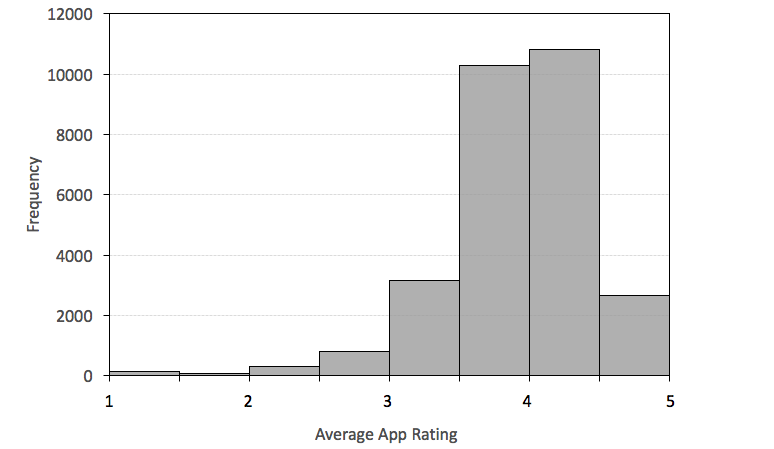
\includegraphics[width=5.3in]{figures/app_rating}
	\caption{移动应用评分的分布情况。横轴表示移动应用在Google Play上的评分,纵轴表示相应评分的移动应用数量。}
\end{figure}
其中13,507(47.79\%)个移动应用获得了超过四星的用户评分,没有一个移动应用获得一星以下的评分。从直方图中可以观察到评分相对较高的移动应用较多,而评分很高(超过四星半)的移动应用又相对较少(9.45\%)。为了更好地比较不同评分的移动应用间使用第三方库的情况,本文根据移动应用的评分情况,将这些移动应用分成四个集合(由于本文的数据集中不包含评分低于一星的移动应用,因而将不做单独讨论):
\begin{itemize}
\item $R_4$:评分超过四星的移动应用,其中包含了13,507个移动应用;
\item $R_3$:评分在三星和四星间的移动应用,其中包含了13,444个移动应用;
\item $R_2$:评分在两星和三星间的移动应用,其中包含了1,104个移动应用;
\item $R_1$:评分低于两星的移动应用,其中包含了206个移动应用。
\end{itemize}

本章将在下文中对这四个评分集合的移动应用进行两两检验,并对每组检验结果进行分析和讨论,具体内容将在3.1节中阐述。此外,本章亦计算了每个集合中移动应用平均所使用的第三方库数量,并以此计算所得结果作为基础进行一一检验,详见3.2节内容。



%%%%%%%%%%%%%%%%%%%%%%%%%%%%%%%%%%%%%%%
%--------------------------------------     个体量检验     --------------------------------------%
%%%%%%%%%%%%%%%%%%%%%%%%%%%%%%%%%%%%%%%
\section{个体量检验}
对于上述所分的四个集合,本文将集合中每个移动应用所使用的第三方库数量作为统计数据,其数据值范围为$[0, +\infty)$。每一组对比检验将对两个集合中所使用的每一个第三方库进行一一检验,即对每一个第三方库,本文将检验两个集合的移动应用所使用的差异,检验结果所得的$P$值作为对原假设的评判依据。本文对第三方库进行了批量检验,为更易发现显著性差异,本文采用了Holm校正方法\cite{holm1979simple},对$P$值进行校正。校正过程是将$n$个检验的$P$值按升序排列,然后分别将这些值除以$n$到1。设$p^{(1)} \leqslant p^{(2)} \leqslant ... \leqslant p^{(n)}$为对第三方库进行$n$个检验后所得的$P$值,且$0 < \alpha < 1$为显著性水平。那么,对$n$个假设的检验以如下方式表示:
\begin{equation}
p^{(1)} > \frac{\alpha}{n}, \quad p^{(2)} > \frac{\alpha}{n-1}, \quad ... , \quad p^{(n)} > \frac{\alpha}{1}
\end{equation}
由于一共有四个评分集合,因此对其进行两两对比检验需要六次检验过程。每组检验校正后的$P$值点分布情况如图3-2所示,其中红色直线表示显著性水平$\alpha$所处位置。从图3-2(a)可以发现,大量$P$值点集中于$\alpha$线下方,即使用这些第三方库的移动应用在两个评分集合$R_4$和$R_3$上表现出了显著差异。但可以看到,$\alpha$线上方同样有大量$P$值点遍布,表明这些第三方库在不同评分的移动应用中并不具有差异性。因为较多第三方库具有较强的通用性,且广泛被移动应用开发者采用,
\begin{figure}
	\centering
	\begin{subfigure}[b]{0.49\textwidth}
		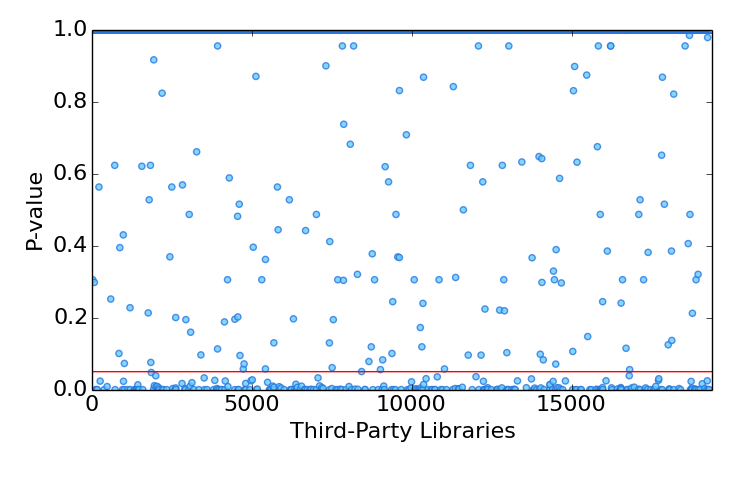
\includegraphics[width=\textwidth]{figures/r4_r3}
		\caption{$R_4$与$R_3$对比检验}
	\end{subfigure}
	\begin{subfigure}[b]{0.49\textwidth}
		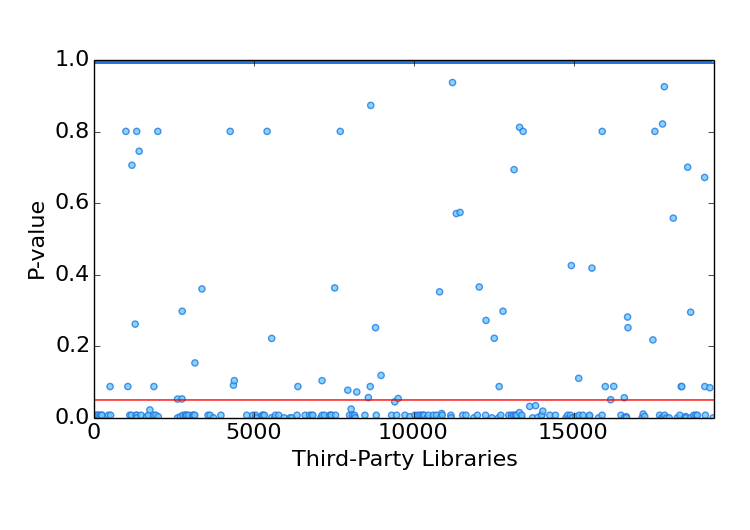
\includegraphics[width=\textwidth]{figures/r4_r2}
		\caption{$R_4$与$R_2$对比检验}
	\end{subfigure}
	\begin{subfigure}[b]{0.49\textwidth}
		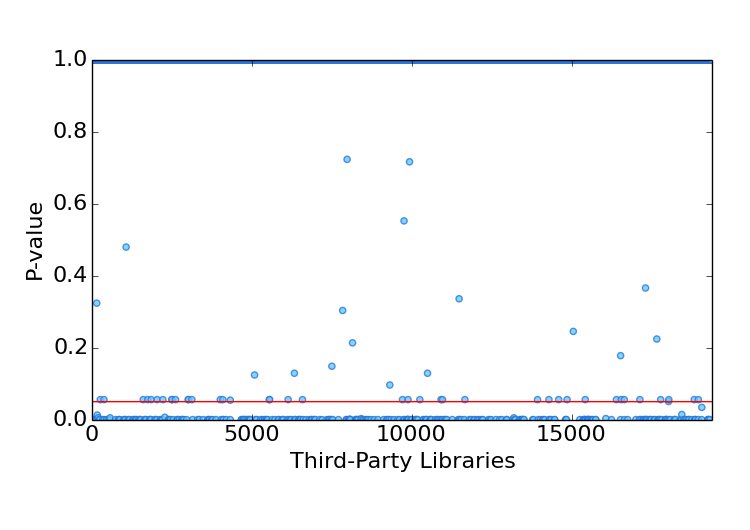
\includegraphics[width=\textwidth]{figures/r4_r0}
		\caption{$R_4$与$R_1$对比检验}
	\end{subfigure}
	\begin{subfigure}[b]{0.49\textwidth}
		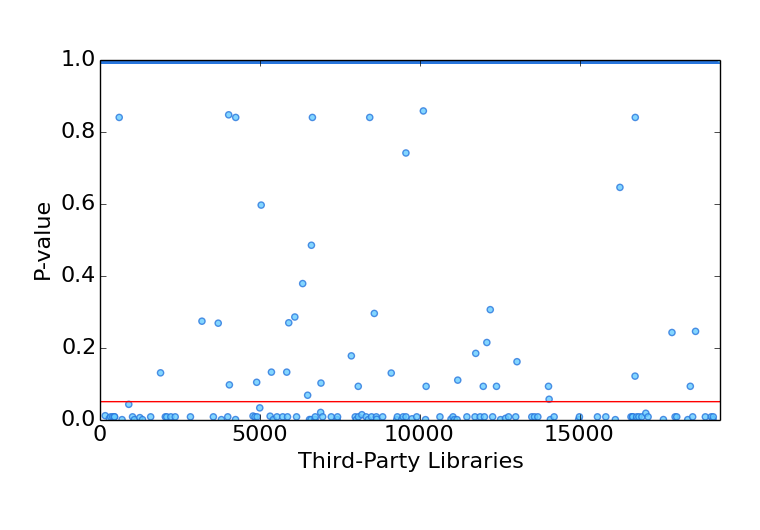
\includegraphics[width=\textwidth]{figures/r3_r2}
		\caption{$R_3$与$R_2$对比检验}
	\end{subfigure}
	\begin{subfigure}[b]{0.49\textwidth}
		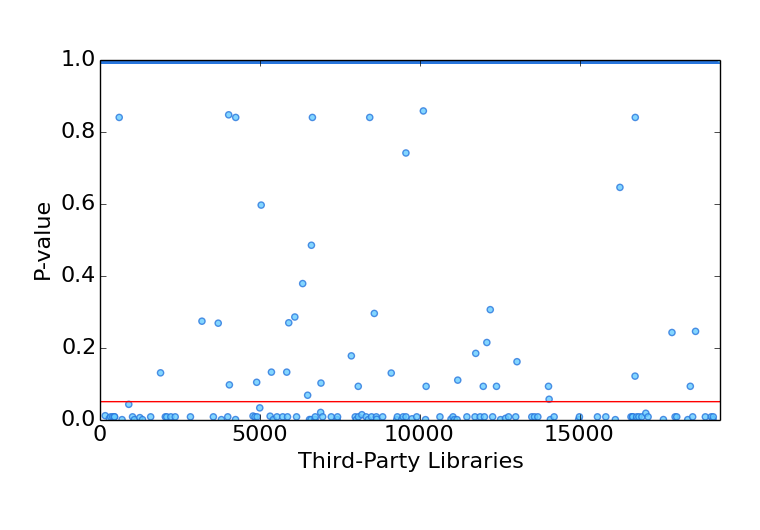
\includegraphics[width=\textwidth]{figures/r3_r2}
		\caption{$R_3$与$R_1$对比检验}
	\end{subfigure}
	\begin{subfigure}[b]{0.49\textwidth}
		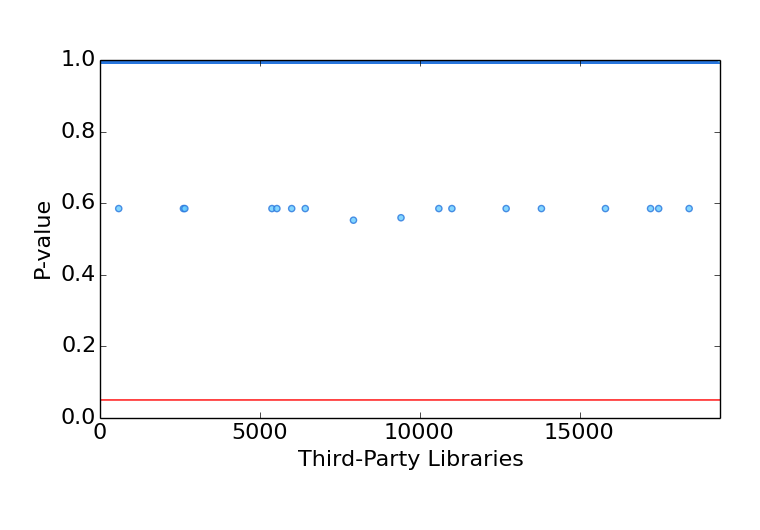
\includegraphics[width=\textwidth]{figures/r2_r0}
		\caption{$R_2$与$R_1$对比检验}
	\end{subfigure}
	\caption{对不同评分集合中所使用的第三方库检验所得的$P$值情况。横轴表示所有被使用的第三方库,纵轴表示不同组检验后所得的$P$值。}
\end{figure}
因而在不同评分集合间不存在明显差异。因此,根据本组对比检验,无法完全拒绝$H0$原假设。图3-2(b)所显示的结果与图3-2(a)类似,同样分别有大量$P$值点分布于$\alpha$线的上下方,但相对而言分布于$\alpha$线上方的$P$值点较为稀疏,说明与上组检验对比,该组表现出了相对较大的差异性。因此,根据$R_4$和$R_2$组检验结果,无法直接对$H0$原假设作出接受或拒绝操作。图3-2(c)所展示的检验结果,相较前两组检验,在$\alpha$线上方分布的$P$值点更为稀疏,说明$R_4$与$R_1$集合间的差异较为显著,虽然依旧无法直接对$H0$原假设作出判断,但从检验结果可以看到明显的差异性。图3-2(d)和图3-2(e)是$R_3$集合分别与$R_2$和$R_1$进行对比检验。从图中可以观察到,这两组检验结果较为相似,均在$\alpha$线下方集中了大量$P$值点,而上方较为稀疏地分布了一些$P$值点。因此,可以观察到$R_3$集合与其他两集合的差异,但无法对$H0$原假设作出明确判断。图3-2(f)表现出了不同的检验结果,可以明显观察到所有的$P$值点都遍布于$\alpha$线上方,说明该组检验中的两个集合并无显著差异。因此,对于$R_2$与$R_1$这一组检验结果,本文接受$H0$原假设,即认为评分在后两类中的移动应用所使用的第三方库没有显著差异。此结论并不与研究问题相悖,因为评分较低的移动应用必然呈现一定的相似性,其所使用的第三方库的数量、质量等方面都较为类似且有待提高。若此两类评分的移动应用在使用第三方库方面与前两类高评分移动应用有明显差异,则从侧面验证了本文所研究问题的根本和必要性,因而本章的检验也将重点关注高评分类别的移动应用与低分类别在统计学上所表现的差异。

通过本节的检验和分析,可以初步观察到第三方库在不同评分的移动应用中的使用情况。其中,大量第三方库在高分($R_3$、$R_4$)与低分($R_1$、$R_2$)间所呈现出来的显著性差异,从而凸显了本文研究问题的意义和价值,也为其他研究者提供了必要的背景定义和数据支撑。下一节将通过对第三方库平均使用情况的检验分析,来说明本文的研究问题和方向。



%%%%%%%%%%%%%%%%%%%%%%%%%%%%%%%%%%%%%%%
%--------------------------------------     均值量检验     --------------------------------------%
%%%%%%%%%%%%%%%%%%%%%%%%%%%%%%%%%%%%%%%
\section{均值量检验}
不同于上一节对每个第三方库进行的检验分析,本节将集中分析每个评分集合中第三方库的平均使用情况。本节分别对四个集合中第三方库的使用情况进行统计,再对统计后结果计算平均值,即集合中每个移动应用平均使用第三方库的数量。对四个集合计算后的第三方库值,采用Mann-Whitney检验方法进行两两配对检验,检验所得的$P$值如下表所示:

\begin{table}
\centering
\caption{不同评分集合的移动应用中第三方库的平均使用情况}
\begin{tabular}{C{1.8in}C{1.2in}C{1in}}
\hline
\hline
Mann-Whitney检验 & $P$值 & 与$\alpha$比较 \\
\hline
$R_4$对比$R_3$ & 0.3076 & > 0.05 \\
$R_4$对比$R_2$ & < 0.0001 & < 0.05 \\
$R_4$对比$R_1$ & 0.0028 & < 0.05 \\
$R_3$对比$R_2$ & < 0.0001 & < 0.05 \\
$R_3$对比$R_1$ & 0.0035 & < 0.05 \\
$R_2$对比$R_1$ & 0.1060 & > 0.05 \\
\hline
\hline
\end{tabular}
\end{table}

从表3-1中可观察到,高评分集合($R_3$、$R_4$)中使用的第三方库与低评分集合($R_1$、$R_2$)有着明显差异。如$R_4$与$R_2$、$R_3$与$R_2$两组对比检验,其$P$值远小于0.0001,与显著性水平$\alpha$相去甚远,说明评分较高的$R_4$和$R_3$集合与低分集合$R_2$在第三方库的平均使用量上有显著差异。同样的,$R_4$与$R_1$、$R_3$与$R_1$两组的对比检验亦有相似的结果,其$P$值均处于$\alpha$线下方,同理可得高评分集合与低评分集合在第三方库使用上的显著差异。根据以上四组对比检验,本文可以拒绝$H0$原假设,即评分高的移动应用在第三方库的使用上与评分低的移动应用有显著差异。从表3-1中亦可发现两组不同的检验结果,即$R_4$与$R_3$、$R_2$与$R_1$两组的$P$值均大于显著性水平。上节讨论了$R_2$与$R_1$对比组的结果,且不影响本文的研究问题。因此,本节将对$R_4$与$R_3$组进行分析,深入了解该两类评分的移动应用在第三方库的使用率上是否有显著差异。

为此,本文对评分大于三星的移动应用进行重新分组,其中每半星分成一个评分类别,处理方式与本章开头相同,分成的四个集合如下:
\begin{itemize}
\item $R_{4.5}$:评分超过四星半的移动应用,其中包含了2,671个移动应用;
\item $R_{4.0}$:评分在四星和四星半间的移动应用,其中包含了10,836个移动应用;
\item $R_{3.5}$:评分在三星半和四星间的移动应用,其中包含了10,291个移动应用;
\item $R_{3.0}$:评分在三星和三星半间的移动应用,其中包含了3,153个移动应用。
\end{itemize}

首先对这四个集合中的第三方库计算平均使用量,其次采用Mann-Whitney检验方法对此四个集合进行两两检验,所得$P$值如下表所示:
\begin{table}
\centering
\caption{不同高评分集合中第三方库的平均使用情况}
\begin{tabular}{C{1.8in}C{1.2in}C{1in}}
\hline
\hline
Mann-Whitney检验 & $P$值 & 与$\alpha$比较 \\
\hline
$R_{4.5}$对比$R_{4.0}$ & 0.0246 & < 0.05 \\
$R_{4.5}$对比$R_{3.5}$ & 0.0014 & < 0.05 \\
$R_{4.5}$对比$R_{3.0}$ & 0.0002 & < 0.05 \\
$R_{4.0}$对比$R_{3.5}$ & 0.0480 & < 0.05 \\
$R_{4.0}$对比$R_{3.0}$ & < 0.0001 & < 0.05 \\
$R_{3.5}$对比$R_{3.0}$ & < 0.0001 & < 0.05 \\
\hline
\hline
\end{tabular}
\end{table}

从表3-2可以观察到,六组检验的所得的$P$值均小于显著性水平$\alpha$。虽然在上文中,检验发现评分集合$R_4$在与评分集合$R_3$对比时,第三方库的使用情况并未体现出统计显著性差异,但将这两类评分集合按半星进行拆分后,其两两对比检验表现出了显著的差异特征,每一组的检验结果都小于$\alpha$。因此,可以拒绝$H0$原假设,并得到以下结果:在高评分集合中,移动应用所使用的第三方库同样表现出了显著的统计学差异。

本节对不同评分的移动应用的第三方库平均使用情况进行检验,分析发现高评分的移动应用在第三方库的使用上与低评分的移动应用表现出了显著差异,而且即便同为较高评分的移动应用,在不同评分层次间同样表现出了明显区别。



%%%%%%%%%%%%%%%%%%%%%%%%%%%%%%%%%%%%%%%
%----------------------------------------     本章小结     ---------------------------------------%
%%%%%%%%%%%%%%%%%%%%%%%%%%%%%%%%%%%%%%%
\section{本章小结}
本章从统计学角度,通过对实际数据的分析,深入探讨了第三方库与移动应用的关系。评分作为移动应用最重要的评价方式之一,是开发者最为关注和在意的方面。因此,任何能够提高移动应用评分的方式都具有现实意义和价值。第三方库作为本文的研究对象,其与移动应用评分的关系是本文研究的基础和出发点。本章的分析,其目的是为了对本文研究问题的依据进行验证。为了比较不同评分的移动应用间使用第三方库的差异,本章将移动应用根据评分高低分成了四个类别,然后对这四个类别的移动应用,分别从第三方库的个体使用量和平均使用量两个方面进行检验分析。检验结果显示了高评分类别的移动应用与低评分类别的显著差异。本章亦对高评分类别的移动应用进行更为细粒度的分析,从一星作为步长减少到半星作为步长,将高评分类别的移动应用分成更小的四个集合。在此基础上,通过两两对比检验,结果表现出与预想一致的结果,即在高评分类别中,就第三方库使用情况,其内部同样具有显著的差异。经过大小对比组的检验分析,本章得出以下结论:\textbf{使用第三方库的移动应用确实具有更高的评分。}此结论回答了本章开始的研究问题,且验证了本文研究问题的依据,为本文的研究工作奠定了基础。本章的检验分析结果可以为其他研究者所用,为其之后在第三方库相关问题的研究中提供数据支撑。